%--------------DOCUMENT--------------------------------------------------------

\documentclass[11pt]{article}
\usepackage{amsmath}
\usepackage{amsfonts}
\usepackage{amssymb}
\usepackage{graphicx}


\title{
DspUnit\\
}
\author{}
\date{}%\fbox{}}
\usepackage{verbatim}
\usepackage{pst-eps}
\begin{document}

\maketitle

%\tableofcontents
% --------------------------------------------------
% -------------  Document Body   -------------------
% --------------------------------------------------


DspUnit is system architectural framework for Digital Signal Processing on SoC. It acts as processor peripheral and can be considered as a DSP accelerator. DspUnit provides various classical signal operators and can be easily extended for specific application purpose. Also, this component is bound to be connected to a processor.

\section{Overview}

DspUnit is intended for block processing (not streaming), hence the operands of each operator are vectors that are stored in Random Access Memory. Basically, the accelerator works on three memories connected through three independant buses. This allows parallel access to data leading to a faster processing.
\begin{figure}
 \centering
 %\includegraphics[width=340]{img/composant.jpg}
 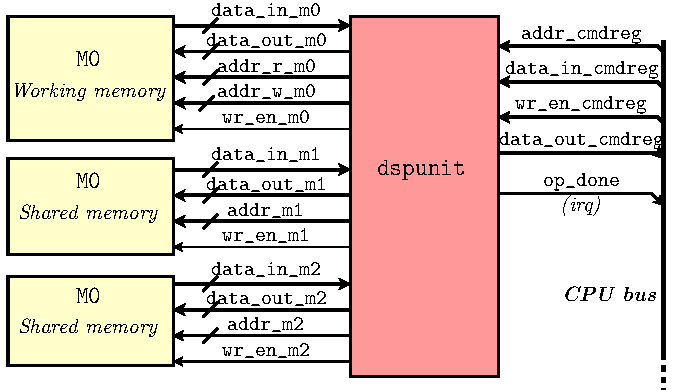
\includegraphics{img/dspunit_inout.pdf}
 \caption{Inputs-Outputs}
\end{figure}
These memories can be shared with external components (processor or other) in order to exchange data. Sharing strategies are developped later.

Operations can be ordered from the processor through the control registers. Processing scheme is sequential in nature but benefits from massive parallelism of ressources unlike in a classical processor. Hence only one operation is active at a time but it can access simultaneously all ressources (memories, ALU, LUT...) and can be pipelined to achieve high efficiency.
\begin{figure}
 \centering
 %\includegraphics[width=340]{img/composant.jpg}
 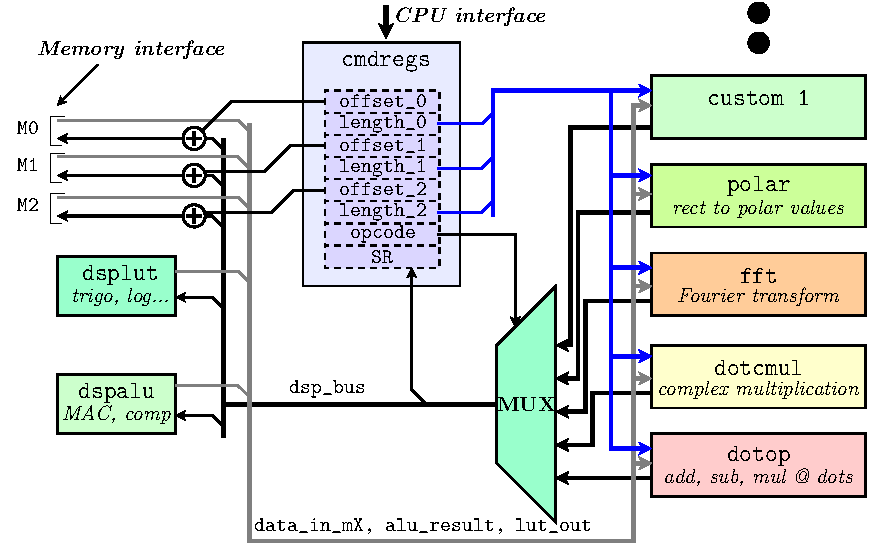
\includegraphics{img/diagramm.pdf}
 \caption{Architecture overview}
\end{figure}

\section{Using DspUnit}

The width of control registers is 16 bits so they can be represented in C-language by the following structure

\begin{tabular}{|c|}
\hline
\begin{minipage}{0.5\textwidth}
\begin{verbatim}
typedef struct{
    uint16_t blank;
    uint16_t startAddr0;
    uint16_t length0;
    uint16_t startAddr1;
    uint16_t length1;
    uint16_t startAddr2;
    uint16_t length2;
    uint16_t opcode;
    uint16_t sr;
}dspcmdreg_t;

extern dspcmdreg_t *dspcmdreg;
\end{verbatim}
\end{minipage}
\\\hline
\end{tabular}


The pointer \texttt{dspcmdreg} must be set to the base address of the control registers depending on your processor memory map.

Then operations can be easil launched from the processor.
The following code launch a copy of 1024 words from memory M1 @ address 0x100 to M2 @ address 0x200:

\begin{tabular}{|c|}
\hline
\begin{minipage}{0.98\textwidth}
\begin{verbatim}
  dspcmdreg->length0 = 1023;
  dspcmdreg->startAddr1 = 0x100;
  dspcmdreg->startAddr2 = 0x200;
  dspcmdreg->opcode = DSPOP_CPMEM | OPFLAG_SRCM1 | OPFLAG_M2;
  dspcmdreg->sr = 2;
\end{verbatim}
\end{minipage}
\\\hline
\end{tabular}

The operation is activated by setting the second bit of status register.



\end{document}



